\iffalse
    \author{EE24BTECH11029}
    \section{ae}
    \chapter{2007}
\fi

\item $\lim_{x \to 0}\frac{\sin x}{e^x x}$
    \begin{enumerate}
        \item $10$
        \item $0$
        \item $1$
        \item $\infty$
    \end{enumerate}
    \item Let the dynamical system be described by the differential equation $2\frac{dy}{dt}+\cos x=0.$ Which of the following differential equations describes this system in a close approximation sense for small perturbation about $x=\frac{\pi}{4}?$
    \begin{enumerate}
        \item $2\frac{dx}{dt}+\sin x=0$
        \item $2\frac{dx}{dt}-\frac{1}{\sqrt{2}}x=0$
        \item $\frac{dx}{dt}+\cos x=0$
        \item $\frac{dx}{dt}+x=0$
    \end{enumerate}
    COMMON DATA FOR QUESTIONS $71,71\&73:$ An airplane designer wants to keep longitudinal static stability margin $\brak{SM}$ within $5\%$ to $15\%$ of mean aerodynamic chard.A wind tunnel test of model showed that for $\bar{X}_{CO}=0.3.\frac{dC}{dC_L}=-0.1.$ Note that the distance from the wing leading edge to the center of the gravity $\brak{X_{CO}}$ has been non-dimensionalized by dividing it with mean aerodynamic chard, $\bar{c}$,such that $\bar{X_{CO}}=\frac{X_{CO}}{\bar{c}}$.Note also that the relation $\frac{dC}{dC_L}=-SM$ holds true for this airplane.
    \item The most forward location of airplane center of gravity permitted to fulfill the designers requirements on longitudinal static margin is
    \begin{enumerate}
        \item $0.35\bar{c}$
        \item $0.25\bar{c}$
        \item $0.15\bar{c}$
        \item $0.52\bar{c}$
    \end{enumerate}
    \item The most of  location of the airplane center of gravity permitted to fulfill designers requirement on longitudinal static stability is
    \begin{enumerate}
         \item $0.35\bar{c}$
        \item $0.25\bar{c}$
        \item $0.52\bar{c}$
        \item $0.67\bar{c}$
    \end{enumerate}
    \item The center of gravity location to have $\frac{d\delta_e}{dC_L}=0$is
    \begin{enumerate}
        \item $0.35\bar{c}$
        \item $0.25\bar{c}$
        \item $0.5\bar{c}$
        \item $0.4\bar{c}$
    \end{enumerate}
     COMMON DATA FOR QUESTIONS $74\&75:$ Consider the spring mass system in the figure below.This system has two degrees of freedom representing the motions of the two masses.

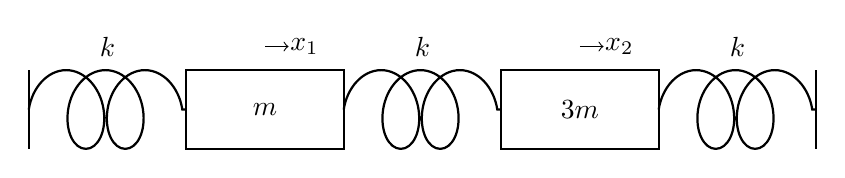
\begin{tikzpicture}

    % Springs
    \draw[thick,decorate,decoration={coil,aspect=0.7,segment length=5mm,amplitude=5mm}] (-2,-0.5) -- (0,-0.5); % Left spring
    \draw[thick,decorate,decoration={coil,aspect=0.7,segment length=5mm,amplitude=5mm}] (2,-0.5) -- (4,-0.5); % Middle spring
    \draw[thick,decorate,decoration={coil,aspect=0.7,segment length=5mm,amplitude=5mm}] (6,-0.5) -- (8,-0.5); % Right spring
    
    % Masses
    \draw[thick] (0,0) rectangle (2,-1); % Left mass m
    \draw[thick] (4,0) rectangle (6,-1); % Right mass 3m

    % Ground supports
    \draw[thick] (-2,0) -- (-2,-1); % Left wall
    \draw[thick] (8,0) -- (8,-1); % Right wall

    % Labels
    \node at (1,-0.5) {$m$}; % Mass m
    \node at (5,-0.5) {$3m$}; % Mass 3m
    \node at (-1,0.3) {$k$}; % Left spring k
    \node at (3,0.3) {$k$}; % Middle spring k
    \node at (7,0.3) {$k$}; % Right spring k

    % Axes and arrows
    \draw[->] (1,0.3) -- (1.3,0.3); % x1 arrow
    \node at (1.5,0.3) {$x_1$}; % x1 label

    \draw[->] (5,0.3) -- (5.3,0.3); % x2 arrow
    \node at (5.5,0.3) {$x_2$}; % x2 label

\end{tikzpicture}


 \item The system shows the following type of coordinate coupling
     \begin{enumerate}
         \item static coupling
         \item dynamic coupling
         \item static and dynamic coupling
         \item no coupling
     \end{enumerate}
     \item The two natural frequencies of system are given as
     \begin{enumerate}
         \item $\sqrt{\frac{4\pm\sqrt{5}}{3}\frac{k}{m}}$
         \item $\sqrt{\frac{4\pm\sqrt{3}}{3}\frac{k}{m}}$
         \item $\sqrt{\frac{4\pm\sqrt{7}}{3}\frac{k}{m}}$
         \item $\sqrt{\frac{4\pm\sqrt{11}}{3}\frac{k}{m}}$
     \end{enumerate}
     STATEMENT FOR LINKED ANSWER QUESTION $76\&77:$ For a piston propeller airplane weighing $20000 N$, the flight testing gat $5 km$ pressure altitude in standard atmosphere gave$ t$ the variation of power required versus true air speed as shown in figure below. The student forgot to label the air speed axis. The maximum climb rate at sea level was calculated to be $4 \frac{m}{s}$. Assume shaft power available to be independent of speed of flight. For piston propeller airplane, it can be assumed that the shaft power available is proportional to ambient density. Values of air density at sea level and at $5 km$ pressure altitude are $1.225 \frac{kg}{m^2}$ and $0.74 \frac{kg}{m^2}$, respectively
     \begin{tikzpicture}
    % Axes
    \draw[->] (0,0) -- (8,0) node[right] {V (True air speed)};
    \draw[->] (0,0) -- (0,6) node[above] {Power required (watts)};
    
    % Labels on y-axis
    \node at (-0.6,1) {$5 \times 10^5$};
    \node at (-0.6,3) {$10 \times 10^5$};
    \node at (-0.6,5) {$15 \times 10^5$};
    
    % Parabolas
    \draw[thick] plot[domain=0.5:4.5, samples=50] (\x, {(\x-2)*(\x-2)/1.2+1}) node[right] {Sea level};
    \draw[thick, dashed] plot[domain=2:6, samples=50] (\x, {(\x-3.5)*(\x-3.5)/1.2+1}) node[right] {5 km};
    
    % Labels for parabolas
    \node at (3,3.5) {Sea level};
    \node at (5.5,3) {5 km};
    
    % Line y = 5
    \draw[dotted] (0,1) -- (8,1);

\end{tikzpicture}
     \item The maximum rate of climb achievable by this airplane at $5 km$ altitude will be
     \begin{enumerate}
         \item $1.65\frac{m}{s}$
         \item $0.51\frac{m}{s}$
         \item $1.43\frac{m}{s}$
         \item $3.65\frac{m}{s}$
     \end{enumerate}
     \item If during the maximum rate of climb at $5km$ altitude,the airplane was flying at an angle of attack of $4$ degree and attitude \brak{pitch} angle of $5$ degrees,what was equivalent airspeed of the airplane ?
     \begin{enumerate}
         \item $40.2\frac{m}{s}$
         \item $63.7\frac{m}{s}$
         \item $130.3\frac{m}{s}$
         \item $20.2\frac{m}{s}$
     \end{enumerate}
     STATEMENT FOR LINKED ANSWER QUESTION $78\&79:$A model wing of rectangular platform has a chord of $0.2 m$ and a span of $1.2 m.$ It has a symmetric airfoil section whose lift curve slope is $0.1$ per degree. When this wing is mounted at $8$ degrees angle of attack in a freestream of $20 \frac{m}{s}$ it is found to develop $35.3 N$ lift when the density of air is $1.225 \frac{kg}{m^3}.$
    \item The lift curve slope of this wing is
    \begin{enumerate}
        \item $0.10$ per deg
        \item $0.092$ per deg
        \item $0.075$ per deg
        \item $0.050$ per deg
    \end{enumerate}
    \item The span efficiency factor of this wing is 
    \begin{enumerate}
        \item $1.0$
        \item $0.91$
        \item $0.75$
        \item $0.63$
    \end{enumerate}
    STATEMENT FOR LINKED ANSWER QUESTION $80\&81:$\\
    Let $F\brak{s}=\frac{\brak{s+10}}{\brak{s+2}\brak{s+20}}$
    \item The partial fraction expansion of $F\brak{s}$ is
    \begin{enumerate}
        \item $\frac{1}{s+2}+\frac{1}{s+20}$
        \item $\frac{5}{s+2}+\frac{2}{s+20}$
        \item $\frac{2}{s+2}+\frac{20}{s+20}$
        \item $\frac{\frac{4}{9}}{s+2}+\frac{\frac{5}{9}}{s+20}$
    \end{enumerate}
    \item The inverse Laplace transform of $F\brak{s}$ is
    \begin{enumerate}
        \item $2e^{-s}+20e^{-3s}$
        \item $\frac{4}{9}e^{-3s}+\frac{5}{9}e^{-4}$
        \item $5e^{-2s}+2e^{-3s}$
        \item $\frac{9}{4}e^{-3s}+\frac{9}{5}e^{-2s}$
    \end{enumerate}
    STATEMENT FOR LINKED ANSWER QUESTION $82\&83:$The equation of motion of a vibrating rod is given by $\frac{\delta^2 u}{\delta x^2}=\frac{1}{e^2}\frac{\delta^2 u}{\delta t^2}.$ Here $u$ is the displacement along the rod and is a function of both position $x$ and time $t$. To find the response of the vibrating rod, we need to solve this equation using boundary conditions and initial conditions.
    \item The boundary conditions needed for fixed at the root $\brak{x=0}$ and free at tip $\brak{x=l}$ are
    \begin{enumerate}
        \item $u\brak{x=0}=0,\frac{\delta u}{\delta x}\brak{x=l}=0$
        \item $u\brak{x=l}=0,\frac{\delta u}{\delta x}\brak{x=l}=0$
        \item $u\brak{x=0}=0,u\brak{x=l}=0$
      \item $\frac{\delta u}{\delta x}\brak{x=0},\frac{\delta u}{\delta x}\brak{x=l}=0$
    \end{enumerate}
    \item The natural frequencies $\omega$ of the fixed-free rod can then be obtained using
    \begin{enumerate}
        \item $\cos\brak{\frac{\omega l}{c}}=0$
        \item $\sin\brak{\frac{\omega l}{c}}=0$
        \item $\cos\brak{\frac{\omega c}{l}}=0$
        \item $\cos\brak{\frac{\omega }{c}}=0$
    \end{enumerate}
    STATEMENT FOR LINKED ANSWER QUESTION $84\&85:$Air enters the compressor of a gas turbine engine with velocity $127 mia,$ density $1.2 \frac{kg}{m^3}$ and stagnation pressure $0.9 MPa.$ Air exits the compressor with velocity $139 \frac{m}{s}$ and stagnation pressure $3.15 MPa.$ Assume that the ratio of specific heats is constant and equal to $1.4.$
    \item The compressor pressure ratio is
    \begin{enumerate}
        \item $0.22$
        \item $0.869$
        \item $0.89$
        \item $0.98$
    \end{enumerate}

